%Fiquemos com Deus e Nossa Senhora!
%Sao Jose de Cupertino rogai por nos!!
% ### Uses XeLaTeX ### %
% ### Needs beamer-master ### %
\documentclass[aspectratio=169]{beamer} %. Aspect Ratio 16:9

\usetheme{AI2} % beamerthemeSprace.sty
\usepackage[portuguese]{babel}
\usepackage[utf8]{inputenc}
\usepackage[T1]{fontenc}
\usepackage{ragged2e,gensymb,bm,amsmath,amssymb}

\DeclareMathOperator*{\argmin}{arg\,min}
\DeclareMathOperator*{\argmax}{arg\,max}
\DeclareMathOperator{\sign}{sgn}

% DATA FOR FOOTER
\date{2021}
\title{- Análise Discriminante Linear}
\author{João Paulo Papa}
\institute{Advanced Institute for Artificial Intelligence (AI2)}

\begin{document}
% ####################################
% FIRST SLIDE 						:: \SliTit{This is the Title of the Talk}{A. B. Name}{Sprace}
% SUB-TITLE SLIDE 					:: \SliSubTit{<title>}{<explanation}
% SUB-SUB-TITLE SLIDE				:: \SliSubSubTit{<title>}{<explanation}
% SLIDE WITH TITLE 					:: \SliT{Title}{Content}
% SLIDE NO TITLE 						:: \Sli{Content} 
% SLIDE DOUBLE COLUMN WITH TITLE 	:: \SliDT{Title}{First Column}{Second Column}
% SLIDE DOUBLE COLUMN NO TITLE 		:: \SliD{First Column}{Second Column}
% SLIDE ADVANCED WITH TITLE 			:: \SliAdvT{Title}{Content}
% SLIDE ADVANCED NO TITLE 			:: \SliAdv{Content}
% SLIDE ADVANCED DOUBLE WITH TITLE 	:: \SliAdvDT{Title}{First Column}{Second Column}
% SLIDE ADVANCED DOUBLE NO TITLE 	:: \SliAdvD{First Column}{Second Column}
% SLIDE BLACK						:: \Black{ <Content> }
% SLIDE WHITE						:: \White{ <Content> }
% ITEMIZATION 						:: \begin{itemize}  \iOn{First} \iTw {Second} \iTh{Third} \end{itemize}
% COMMENT TEXT				 		:: \note{<comment>}
% SECTION 							:: \secx{Section} | \secxx{Sub-Section}
% BOLD SPRACE COLOR				:: \bfs{<text>}
% TABLE OF CONTENT					:: \tocitem{<title>}{<content>}
% LEFT ALIGN EQUATION				:: \begin{flalign*}  & <equation> &   \end{flalign*}
% CENTER ALIGN EQUATION	S			:: \begin{gather*} <equations>  \end{gather*}
% SLASH								:: \slashed{<>}
% BAR								:: \barr{<letter>} instead of \bar{<letter>}
% THEREFORE						:: use \portanto (larger and bold}
% 2 or 3 MATH SYMBOLS				:: \overset{<up>}{<down>} &  \underset{<below>}{\overset{<above>}{<middle>}}  
% INSERT TEXT IN FORMULA			:: \ins{<text>}
% EXERCISE							:: \exe{<exercise #>}{<exercise text>}
% SUGGESTED READING BOX			:: \sug{<references>}
% CITATION							:: \cittex{<citation>}
% CITATION DOUBLE COLUMN 			:: \cittexD{<citation>}
% TEXT POSITION						:: \texpos{<Xcm>}{<Ycm>}{<text>} origin = center of slide : x right | y down
% REFERENCE AT BOTTOM  S/D SLIDE		:: \refbotS{<reference>} \refbotD{<reference>}
% HIDDEN SLIDE						:: \hid
% COLOR BOX 						:: \blu{blue} + \red{rec} + \yel{yellow} + \gre{green} + \bege{beige}
% FRAME 							:: \fra{sprace} \frab{blue} \frar{red} + \fray{yellow} + \frag{green}		
% FIGURE 							:: \img{X}{Y}{<scale>}{Figure.png} 
% FIGURE							:: \includegraphics[scale=<scale>]{Figures/.png}
% FIGURE DOUBLE SLIDE NO TITLE		::  \img{-4}{0.5}{<scale>}{Figure.png} % Image 1st half
%									::  \img{4}{0.5}{<scale>}{Figure.png} % Image 2nd half
% FIGURE DOUBLE SLIDE WITH TITLE		::  \img{-4}{0}{<scale>}{Figure.png} % Image 1st half
%									::  \img{4}{0}{<scale>}{Figure.png} % Image 2nd half
% INCLUDING SWF (Flash)				:: \usepackage{media9} and \includemedia >> USE ACROBAT <<
%%%%%%%%%%%%%%%%%%%%%%%%%%%%%%%%%%%%%%%%%%%%%%%%%%
% ###############################################################################
% FIRST SLIDE
\SliTit{{\LARGE Análise Discriminante Linear}}{Advanced Institute for Artificial Intelligence -- AI2}{https://advancedinstitute.ai}
%%%%%%%%%%%%%%%%%%%%%%%%%%%%%%%%%%%%%%%%%%%%%%%%%%
% ###############################################################################
% SLIDE SUB-TITLE
%\SliSubTit{Sub-Title}{Description}{}
%%%%%%%%%%%%%%%%%%%%%%%%%%%%%%%%%%%%%%%%%%%%%%%%%%
% ###############################################################################
%\SliSubSubTit{Sub-Sub-Title}{Description}
 %%%%%%%%%%%%%%%%%%%%%%%%%%%%%%%%%%%%%%%%%%%%%%%%%%


\SliT{Introdução}{

\justifying Análise Discriminante Linear, do inglês \emph{Linear Discriminant Analysis} - LDA, é uma técnica \textbf{supervisionada} que objetiva \textbf{maximizar a separabilidade} entre as classes. A ideia é gerar agrupamentos em que a distância intraclasse (elementos de mesma classe) seja pequena, enquanto que a distância interclasse (elementos de classes distintas) seja grande. \textbf{Queremos, então, gerar agrupamentos compactos e distantes.}

\begin{center}
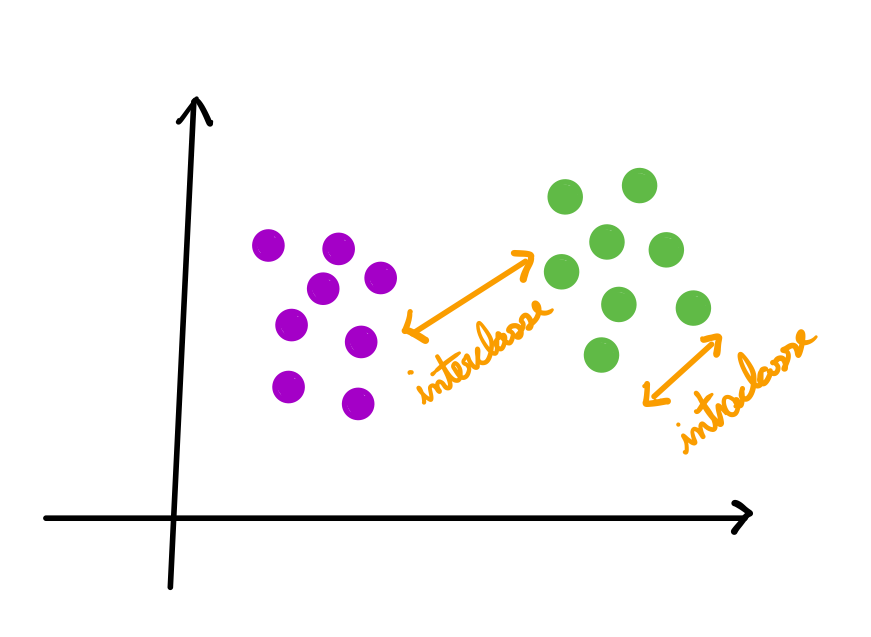
\includegraphics[scale=0.19]{./figs/LDA_Fig1.png}
\end{center}
}

\Sli{
\justifying Seja ${\cal X}=\{(\bm{x}_1,y_1),(\bm{x}_2,y_2),\ldots,(\bm{x}_z,y_z)\}$ um conjunto de dados rotulado tal que $\bm{x}_i\in\mathbb{R}^n$. Temos que ${\cal X}_1\subset {\cal X}$ e ${\cal X}_2\subset {\cal X}$ representam duas partições que denotam os conjuntos de treinamento e teste, respectivamente. Ademais, seja ${\cal Y}=\{\omega_1,\omega_2,\ldots,\omega_c\}$ o conjunto de rótulos	possíveis. Em nosso exemplo, vamos assumir que temos apenas duas classes, isto é, $\omega_1$ e $\omega_2$.

\justifying Podemos calcular as médias de cada agrupamento da seguinte forma:

\begin{equation}\nonumber
\bm{\mu}_1 = \frac{1}{m_1}\sum_{\bm{x}_i\in\omega_1}\bm{x}_i \text{\ \ \ \ e\ \ \ \ } \bm{\mu}_2 = \frac{1}{m_2}\sum_{\bm{x}_j\in\omega_2}\bm{x}_j,
\end{equation}
\justifying em que $m_1$ e $m_2$ correspondem ao número de amostras de treinamento das classes $1$ e $2$, respectivamente. Já $\bm{\mu}_1$ e $\bm{\mu}_2$ denotam os centros dos agrupamentos das amostras das classes $1$ e $2$, respectivamente.
}

\Sli{
\justifying \underline{Objetivo:} dado um conjunto de treinamento ${\cal X}_1$, achar um vetor direção $\bm{w}\in\mathbb{R}^n$ de tal forma que, quando projetarmos nossas amostras nesta direção, maximizaremos a sua separabilidade.

\justifying Sejam $\hat{\bm{\mu}_1}$ e $\hat{\bm{\mu}_2}$ as médias dos dados das classes $1$ e $2$, respectivamente, projetados na direção $\bm{w}$:

\begin{minipage}{0.57\textwidth}
\begin{align}\nonumber
	\hat{\bm{\mu}_1} &= \frac{1}{m_1}\sum_{\bm{x}_i\in\omega_1}\bm{w}^T\bm{x}_i \\
	&= \underbrace{\bm{w}^T}_{\text{constante}}\left(\frac{1}{m_1}\sum_{\bm{x}_i\in\omega_1}\bm{x}_i\right)\\
	&= \bm{w}^T\bm{\mu}_1.\nonumber
\end{align}
\end{minipage}%%% to prevent a space
\begin{minipage}{0.42\textwidth}
\begin{align}\nonumber
	\hat{\bm{\mu}_2} &= \frac{1}{m_2}\sum_{\bm{x}_j\in\omega_2}\bm{w}^T\bm{x}_j \\
	&= \underbrace{\bm{w}^T}_{\text{constante}}\left(\frac{1}{m_2}\sum_{\bm{x}_j\in\omega_2}\bm{x}_j\right)\\
	&= \bm{w}^T\bm{\mu}_2.\nonumber
\end{align}

\null
\par\xdef\tpd{\the\prevdepth}
\end{minipage}
}

\Sli{
\justifying Um critério interessante seria maximizar a diferença entre as médias projetadas, ou seja, $|\hat{\bm{\mu}}_1-\hat{\bm{\mu}}_2|$:

\begin{minipage}{0.41\textwidth}
\begin{center}
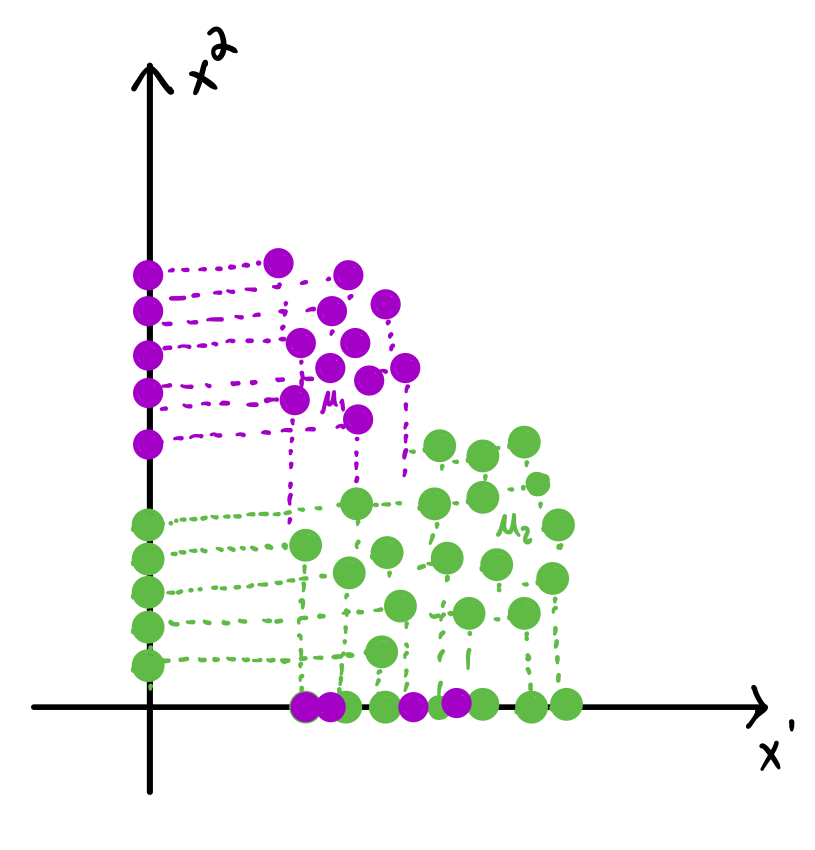
\includegraphics[scale=0.19]{./figs/LDA_Fig2.png}
\end{center}
\end{minipage}%%% to prevent a space
\begin{minipage}{0.42\textwidth}
Neste exemplo, a distância entre as médias é maior no eixo $x^1$, mas a separabilidade é maior no eixo $x^2$.
\null
\par\xdef\tpd{\the\prevdepth}
\end{minipage}

Por que isto ocorre? A abordagem acima não leva em consideração a variância, ou seja, o \textbf{espalhamento} entre as classe.
}

\Sli{
\justifying Dado o nosso conjunto de dados ${\cal X}=\{(\bm{x}_1,y_1),(\bm{x}_2,y_2),\ldots,(\bm{x}_z,y_z)\}$, temos que sua média amostral é dada por:

\begin{equation}
	\bm{\mu} = \frac{1}{z}\sum_{i=1}^z\bm{x}_i,
\end{equation}
e o seu espalhamento (\emph{scatter}) é calculado como segue:

\begin{equation}
	\bm{s}^2 = \sum_{i=1}^z(\bm{x}_i-\bm{\mu})^2.
\end{equation}

Ademais, seja $\hat{\bm{x}}_i=\bm{w}^T\bm{x}_i$ a projeção da amostra $\bm{x}_i$ na direção do vetor $\bm{w}$.
}

\Sli{
\justifying Temos que os espalhamentos no espaço projetado para as classes $\omega_1$ e $\omega_2$ são definidos como segue:

\begin{equation}
\label{e.espalhamento_class_1}
	\hat{\bm{s}}_1^2 = \sum_{\hat{\bm{x}}_i\in\omega_1}(\hat{\bm{x}}_i-\hat{\mu}_1)^2,
\end{equation}
e
\begin{equation}
\label{e.espalhamento_class_2}
	\hat{\bm{s}}_2^2 = \sum_{\hat{\bm{x}}_j\in\omega_2}(\hat{\bm{x}}_j-\hat{\mu}_2)^2.
\end{equation}
\justifying Assim, desejamos \textbf{maximizar a distância entre as médias} e \textbf{minimizar o espalhamento entre as classes}. O Critério de Fisher atende à esta nossa exigência.
}

\Sli{
\justifying Temos, então, que maximizar o Critério de Fisher, dado por:

\begin{equation}
	J(\bm{w}) = \frac{(\hat{\mu}_1-\hat{\mu}_2)}{\hat{\bm{s}}_1^2+\hat{\bm{s}}_2^2}.
\end{equation}
Desta forma, queremos encontrar o vetor $\bm{w}$ que maximiza o critério, acima, ou seja:

\begin{equation}
	w^\ast = \argmax_{\bm{w}}J(\bm{w}).
\end{equation}
No entanto, precisamos reescrever tanto o numerador quanto o denominador em termos de $\bm{w}$.
}

\Sli{
\justifying Antes da projeção, podemos obter as matrizes de espalhamento (\emph{scatter}) das classes $\omega_1$ e $\omega_2$ como segue:

\begin{equation}
	\bm{S}_1 = \sum_{\bm{x}_i\in\omega_1}(\bm{x}_i-\bm{\mu}_1)(\bm{x}_i-\bm{\mu}_1)^T
\end{equation}
e
\begin{equation}
	\bm{S}_2 = \sum_{\bm{x}_j\in\omega_2}(\bm{x}_j-\bm{\mu}_2)(\bm{x}_j-\bm{\mu}_2)^T.
\end{equation}
Seja $S_A = S_1+S_2$ a matriz de espalhamento \textbf{intraclasse}. Podemos reescrever a Equação 5 como segue:

\begin{equation}
	\hat{\bm{s}}_1^2 = \sum_{\hat{\bm{x}_i}\in\omega_1}(\hat{\bm{x}_i}-\hat{\bm{\mu}_1})^2 = \sum_{\hat{\bm{x}_i}\in\omega_1}(\bm{w}^T\bm{x}_i-\bm{w}^T\bm{\mu}_1)^2 = \sum_{\hat{\bm{x}_i}\in\omega_1}[\bm{w}^T(\bm{x}_i-\bm{\mu}_1)]^T[\bm{w}^T(\bm{x}_i-\bm{\mu}_1)].
\end{equation}
}

\Sli{
\justifying Rearranjando os termos, temos que:

\begin{align}\nonumber
	\hat{\bm{s}}_1^2 &= \sum_{\hat{\bm{x}_i}\in\omega_1}[\bm{w}^T(\bm{x}_i-\bm{\mu}_1)]^T[\bm{w}^T(\bm{x}_i-\bm{\mu}_1)]\\
	&= \sum_{\hat{\bm{x}_i}\in\omega_1}[(\bm{x}_i-\bm{\mu}_1)^T\bm{w}]^T[(\bm{x}_i-\bm{\mu}_1)^T\bm{w}]\\\nonumber
	&= \sum_{\hat{\bm{x}_i}\in\omega_1}\bm{w}^T(\bm{x}_i-\bm{\mu}_1)(\bm{x}_i-\bm{\mu}_1)^T\bm{w}\\\nonumber
	&= \bm{w}^T\underbrace{\sum_{\hat{\bm{x}_i}\in\omega_1}(\bm{x}_i-\bm{\mu}_1)(\bm{x}_i-\bm{\mu}_1)^T}_{\bm{S}_1}\bm{w}\\\nonumber
	&= \bm{w}^T\bm{S}_1\bm{w}.
	\end{align}
}

\Sli{
\justifying De maneira análoga, podemos escrever:

\begin{equation}
	\hat{\bm{s}}_2^2 = \bm{w}^T\bm{S}_2\bm{w}.
\end{equation}

\justifying Substituindo-se as Equações 12 e 13 na Equação 7, temos que:

\begin{equation}
	J(\bm{w}) = \frac{\hat{\bm{\mu}}_1-\hat{\bm{\mu}}_2}{\hat{\bm{s}}_1^2-\hat{\bm{s}}_2^2} = \frac{\hat{\bm{\mu}}_1-\hat{\bm{\mu}}_2}{\bm{w}^T\bm{S}_1\bm{w}-\bm{w}^T\bm{S}_2\bm{w}} = \frac{\hat{\bm{\mu}}_1-\hat{\bm{\mu}}_2}{\bm{w}^T(\underbrace{\bm{S}_1+\bm{S}_2}_{\bm{S}_A})\bm{w}} = \frac{\hat{\bm{\mu}}_1-\hat{\bm{\mu}}_2}{\bm{w}^T\bm{S}_A\bm{w}},
\end{equation}
a qual é uma forma quadrática em $\bm{w}$.
}

\Sli{
\justifying Seja, agora, $\bm{S}_B$ a matriz de espalhamento interclasses, que pode ser definida como segue:

\begin{equation}
	\bm{S}_B = (\bm{\mu}_1-\bm{\mu}_2)(\bm{\mu}_1-\bm{\mu}_2)^T,
\end{equation}
a qual mede a separação entre os vetores média antes da projeção. Note que o numerador da Equação 14 pode ser expressa como:

\begin{equation}
	(\bm{\mu}_1-\bm{\mu}_2)^2 = (\bm{w}^T\bm{\mu}_1-\bm{w}^T\bm{\mu}_2)^2 = [\bm{w}^T(\bm{\mu}_1-\bm{\mu}_2)]^T[\bm{w}^T(\bm{\mu}_1-\bm{\mu}_2)].
\end{equation}
Rearranjando os produtos internos, temos que:
\begin{equation}
	(\bm{\mu}_1-\bm{\mu}_2)^2 = [(\bm{\mu}_1-\bm{\mu}_2)\bm{w}^T]^T[(\bm{\mu}_1-\bm{\mu}_2)\bm{w}^T]=\bm{w}^T(\bm{\mu}_1-\bm{\mu}_2)(\bm{\mu}_1-\bm{\mu}_2)^T\bm{w} = \bm{w}^T\bm{S}_B\bm{w}.
\end{equation}
}

\Sli{
\justifying Podemos reescrever o numerador da Equação 14 utilizando o resultado da Equação 17, obtendo uma expressão final para o Critério de Fisher:

\begin{equation}
	J(\bm{w}) = \frac{\bm{w}^T\bm{S}_B\bm{w}}{\bm{w}^T\bm{S}_A\bm{w}}.
\end{equation}

Precisamos, agora, maximizar a Equação 18 com relação à $\bm{w}$, ou seja, calculamos $\frac{\partial J(\bm{w})}{\partial\bm{w}}$, resultando em uma equação fechada para o cálculo de $\bm{w}$, dada por:

\begin{equation}
	\bm{w}^\ast = \bm{S}_{A}^{-1}(\bm{\mu}_1-\bm{\mu}_2),
\end{equation}
que é, basicamente, a diferença entre as médias modulada pela matriz de espalhamento.
}

\SliT{Análise Discriminante Múltipla}{

\justifying Suponha, agora, que tenhamos um problema de classificação por múltiplas classes, isto é, ${\cal Y}=\{\omega_1,\omega_2,\ldots,\omega_c\}$. Neste caso, podemos reduzir a dimensionalidade do espaço original para, no máximo, $c-1$ classes. Temos que a operação de transformação é dada por:

\begin{equation}
	\hat{\bm{x}_i} = \bm{W}^T\bm{x}_i,
\end{equation}
em que, novamente, $\bm{x}_i\in\mathbb{R}^n$ e $\bm{W}\in\mathbb{R}^{n\times d}$ é uma matriz de projeção para um espaço com $d<c$ dimensões. Temos que cada coluna de $\bm{W}$ é uma direção ortogonal $\bm{w}_j$ .
}

\Sli{
\justifying Relembrando que temos as seguintes definições:

\begin{itemize}
	\item $m_i$: número de elementos do conjunto de treinamento da classe $\omega_i$.
	\item $\bm{\mu}_i$: média dos elementos da classe classe $\omega_i$.
	\item $\bm{\mu}$: média global, isto é, de todo o conjunto de treinamento.
\end{itemize}
A função objetivo (Critério de Fisher) a ser maximizada é dada por:

\begin{equation}
	J(\bm{W}) = \frac{|\bm{W}^T\bm{S}_B\bm{W}|}{|\bm{W}^T\bm{S}_A\bm{W}|},
\end{equation}
em que $|\cdot|$ calcula o determinante de uma matriz.
}

\Sli{
\justifying Já as matrizes $\bm{S}_A$ e $\bm{S}_B$ são calculadas como segue:

\begin{equation}
	\bm{S}_A = \sum_{i=1}^c\bm{S}_i = \sum_{i=1}^c\sum_{\bm{x}_j\in\omega_i}(\bm{x}_j-\bm{\mu}_i)(\bm{x}_j-\bm{\mu}_i)^T,
\end{equation}
em que $\bm{S}_i$ representa a matriz de espalhamento da classe $\omega_i$, e

\begin{equation}
	\bm{S}_B = \sum_{i=1}^cm_i(\bm{\mu}_i-\bm{\mu})(\bm{\mu}_i-\bm{\mu})^T.
\end{equation}
Pode-se mostrar que o posto (rank) da matriz $\bm{S}_B$ é $c-1$, ou seja, o número de linhas ou colunas linearmente independentes é limitado superiormente à $c-1$ (número de direções discriminantes do método).
}

\Sli{
\justifying A condição para maximização de nosso Critério de Fisher é dada por:

\begin{equation}\nonumber
	\frac{\partial J(\bm{W})}{\partial \bm{W}} = 0.
\end{equation}
Resolvendo analiticamente a equação acima, chegamos na seguinte formulação:

\begin{equation}
	(\bm{S}_B\bm{W}) = \lambda\bm{S}_A\bm{W}.
\end{equation}
Caso $\bm{S}_A$ admita inversa, temos que:

\begin{equation}
	(\bm{S}_A^{-1}\bm{S}_B)\bm{W} = \lambda\bm{W}.
\end{equation}
Para resolver o problema, basta selecionarmos, no máximo, $c-1$ autovetores de $(\bm{S}_A^{-1}\bm{S}_B)$ associados aos $c-1$ maiores autovalores.
}

\Sli{
\justifying Algumas limitações do LDA:

\begin{itemize}
	\item Não é interessante para problemas com poucas classes e muitas características.
	\item Quanto a média das classes são muito próximas, o numerador da Equação 7 tende a $0$.
	\item Situações em que a função de custo (objetivo) assume valores muito altos (classes com formas não lineares).
\end{itemize}
}

\end{document}